\section{Cryptanalysis of GGH signatures}
While the GGH trapdoor is based on CVP, a known hard lattice problem, the public-key cryptosystem and the signature schemes proposed by GGH in their original form are not given formal security proofs. Indeed, in 1999 the proposed public-key cryptosystem was cryptanalyzed by Phong Q. Nguyen \cite{nguyen1999cryptanalysis}, who successfully solved the GGH encryption challenges posed by the original authors. Later, Nguyen and Oded Regev published cryptanalysis of the GGH signature scheme \cite{nguyen2006learning}, which exploited the signature scheme's design flaws that caused message-signature pairs to leak information about the secret key.

In this section we will discuss the cryptanalysis of the GGH signature scheme by first summarizing the key results from Nguyen and Regev, then provide an implementation that simulate the key-recovery attack.

\subsection{Learning a hidden parallelepiped}
As Nguyen and Regev pointed out, the main weakness of the GGH signature scheme lies in the fact that messages are hashed uniformly into (a finite subset) of $\mathbb{Z}^n$ and each signature is exactly the unique lattice point $\mathbf{v} \in \mathcal{L}(R)$ (where $R$ is the secret basis) whose centered fundamental parallelepiped $\mathbf{v} + \mathcal{C}(R) = \{\mathbf{v} + R\mathbf{x} \mid \mathbf{x} \in [-\frac{1}{2}, \frac{1}{2})\}$ contains the hashed message. This means that for each message-signature pair $(\mathbf{m}, \mathbf{\sigma})$, their difference $\mathbf{m} - \mathbf{\sigma}$ is a uniform sample of the centered fundamental parallelepiped $\mathcal{C}(R)$. The cryptanalysis of the GGH signature scheme is thus an algorithm that approximates the basis spanning $\mathcal{C}(R)$, which Nguyen and Regev termed the \textit{hidden parallelepiped problem} (HPP).

\begin{figure}[h]
    \centering
    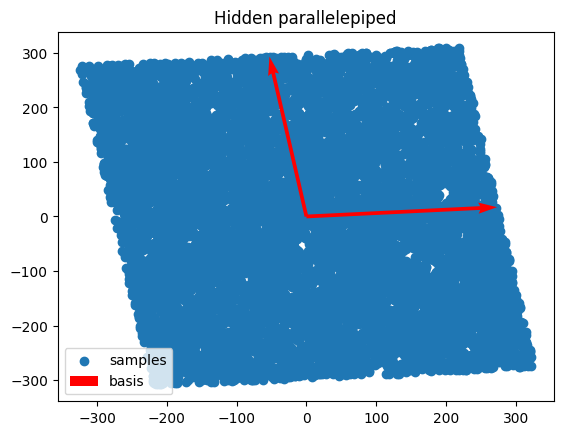
\includegraphics[width=0.7\textwidth]{hidden-parallelepiped.png}
    \caption{message-signature pairs reveal the parallelepiped spanned by the secret basis}
\end{figure}

\begin{definition}
    let $V = [\mathbf{v}_1, \mathbf{v}_2, \ldots, \mathbf{v}_n]$ be a full-rank matrix in $\mathbb{R}^{n \times n}$ and let $\mathcal{P}(V) = \{V\mathbf{x} \mid \mathbf{x} \in [-1, 1]^n\}$ denote the parallelepiped spanned by $V$. The \textbf{hidden parallelepiped problem} asks to approximate the vectors of $V$ using a polynomial-bound number of uniform samples in the parallelepiped
\end{definition}

The main algorithm for solving HPP first approximates the Gram matrix of the basis of the parallelepiped, which can then be used to approximate a linear transformation that maps the parallelepiped to a hypercube (which is a parallelepiped with an orthonormal basis). The basis of the hypercube can be approximated using a gradient descent, and the basis of the parallelpiped can be computed by inverting the hypercube transformation.

Learning the basis of a hypercube can be efficiently done through a gradient descent on the fourth moment of a uniform distribution on the hypercube:

\begin{definition}
    Given basis $V = [\mathbf{v}_1, \ldots, \mathbf{v}_n] \in \mathbf{r}^{n \times n}$, define the k-th moment of a uniform distribution on $\mathcal{P}(V)$ over a vector $\mathbf{w} \in \mathbb{R}^n$ as

    $$
    \operatorname{mom}_{V, k}(\mathbf{w}) = \exp[
        \langle \mathbf{u}, \mathbf{w} \rangle^k
    ]
    $$

    Where $\mathbf{u}$ is uniform sample from $\mathcal{P}(V)$
\end{definition}

Gradient descent on the fourth moment of the hypercube is an appropriate algorithm due to the following lemma:

\begin{lemma}
    Given basis $V = [\mathbf{v}_1, \ldots, \mathbf{v}_n] \in \mathbb{R}^{n \times n}$ of a unit hypercube, there exists a unique global minimum of $\operatorname{mom}_{V, 4}(\mathbf{w})$ achieved at $\pm\mathbf{v}_1, \pm\mathbf{v}_2, \ldots, \pm\mathbf{v}_n$ and no other local minimum
\end{lemma}

\begin{algorithm}
\caption{Learning a hidden parallelepiped}
\begin{algorithmic}[1]
    \State Approximate $G^\prime \approx V^\intercal V$
    \State Compute the Cholesky factor $L$ of $G^{-1}$: $G^{-1} = LL^\intercal$
    \State Transform the parallelepiped samples into hypercube samples $\mathbf{x} \in \mathcal{P}(V) \mapsto \mathbf{x}L$
    \State Approximate the basis of the hypercube $C^\prime = [\mathbf{c}_1, \mathbf{c}_2, \ldots, \mathbf{c}_n]$
    \State Transform the hypercube basis back to parallelepiped basis $\mathbf{v} \leftarrow \mathbf{c}L^{-1}$
\end{algorithmic}
\end{algorithm}

\begin{algorithm}\label{algo-learning-hypercube}
\caption{Learning a hidden hypercube}
\begin{algorithmic}[1]
    \State Choose some initial unit vector for $\mathbf{w}$
    \While{True}
        \State Approximate the gradient $\nabla \operatorname{mom}_{V, 4}(\mathbf{w})$ of the fourth moment at $\mathbf{w}$
        \State Denote $\mathbf{w}^\prime \leftarrow \mathbf{w} - \delta \nabla \operatorname{mom}_{V, 4}(\mathbf{w})$, then normalize $\mathbf{w}^\prime$
        
        \If{$\operatorname{mom}_{V, 4}(\mathbf{w}^\prime) 
            > \operatorname{mom}_{V, 4}(\mathbf{w})$}
            \State return $\mathbf{w}$
        \Else
            \State Replace $\mathbf{w}$ with $\mathbf{w}^\prime$
        \EndIf 
    \EndWhile
\end{algorithmic}
\end{algorithm}

\subsection{Experimental results}
The GGH signature scheme and the HPP learning algorithm were implemented using Python. The matrix arithmetics, including dot products, matrix inversion, and Cholesky factorization, are all computed using numpy 1.26.2. A demo of the cryptanalysis is available on GitHub \footnote{https://github.com/xuganyu96/lattice-crypto-notes/blob/main/gghattack/demo.ipynb}.

In this implementation, the secret basis is generated using the formula $R \leftarrow kI + R^\prime$, where $R^\prime$ is uniformly sampled from $\{-l, -l + 1, \ldots, l-1, l\}^{n \times n}$, $l = 100$, and $k = \lfloor \sqrt{n} \cdot l \rceil$. Messages are uniformly sampled from $\mathbf{m} \leftarrow \{-99999, \ldots, 99999\}^n$, and signatures are computed using simple rounding algorithm $\sigma \leftarrow R \lfloor R^{-1}\mathbf{m} \rceil$. Note that we can also use nearest plane to compute the signature, although with that we will be learning the basis of the orthogonal parallelepiped spanned by $B^\ast$.

We take advantage of the following lemma when approximating the Gram matrix:

\begin{lemma}
    Given a parallelepiped $\mathcal{P}(V)$ and a uniformly sampled vector $\mathbf{v} \leftarrow \mathcal{P}(v)$:

    $$
    \exp[\mathbf{v}\mathbf{v}^\intercal] = \frac{1}{3}VV^\intercal
    $$
\end{lemma}

We also compute the moment and its gradient using the samples through the following approximation:

$$
\mathop{\text{mom}}_{V,k}(\mathbf{w}) \approx \frac{1}{n}\sum_{\mathbf{u} \in S} (\mathbf{u}^\intercal\mathbf{w})^k
$$

$$
\frac{\partial}{\partial\mathbf{w}}
\bigg\lbrack
    \mathop{\text{mom}}_{V,k}(\mathbf{w})
\bigg\rbrack
\approx \frac{k}{n}
\sum_{\mathbf{u} \in S} \bigg(
(\mathbf{u}^\intercal\mathbf{w})^{k-1}\mathbf{u}
\bigg)
$$

Following the recommendation of Nguyen and Regev, the rate of the gradient descent is set to $\delta = 0.7$. For initial positions of $\mathbf{w}$, we iterated through the columns of the identity matrix $I_n$, and we found that they each descended into a distinct basis. In other words, running gradient descent on each of these initial positions allowed us to approximate all secret basis vectors.

While this implementation did not recover the exact value of the secret basis, the approximated secret basis is numerically very close to the true secret basis. We meansured the quality of the basis by computing the determinant of $B^{-1}B^\prime$ where $B^\prime$ is the approximated basis: the closer this determinant is to 1, the better $B^\prime$ is an approximation of $B$.

On an M1 MacBook Air, approximating the secret basis at dimension $n = 80$ with 200000 pairs of message-signature pair could be done in only a few minutes. I could not reliably approximate secret basis of higher dimensions due to integer overflow limitations of numpy, though using C++ with appropriate big integers, the original authors were able to recover secret basis with more than 400 dimensions using 200000 samples.

\begin{figure}[h]
    \centering
    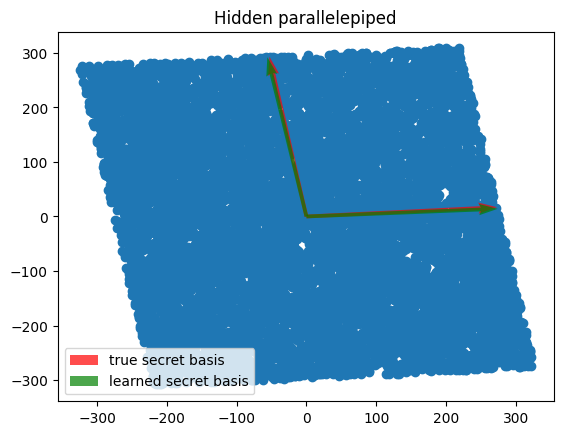
\includegraphics[width=0.7\textwidth]{learned-hpp.png}
    \caption{Recovering a strong approximation of the secret basis}
\end{figure}